\chapter{Methodology}
\ifpdf
    \graphicspath{{Chapter3/Chapter3Figs/PNG/}{Chapter3/Chapter3Figs/PDF/}{Chapter3/Chapter3Figs/}}
\else
    \graphicspath{{Chapter3/Chapter3Figs/EPS/}{Chapter3/Chapter3Figs/}}
\fi

\section{Multi-Task-Learning (MTL) model}\label{MTL}
\vspace*{3mm}
As depicted in Figure \ref{MTL_fig}, the segmentation-classification MTL model performs multiclass segmentation to get the detected tumour region from the MRI, and also gives the prediction probability of the binary classification of the glioblastoma being methylated/unmethylated. (Results are summarized in section \ref{MTL_results})
\vspace*{3mm}

We only need an accurate tumour localization in the segmentation step, so we change the tumour masks from being 4-class of labels \{0,1,2,3\} to being a binary mask of labels \{0,1\}. This is done by simply equating the non-zero pixel labels to 1. The below figure shows some examples:
\vspace*{4mm}
\begin{figure}[H]
  \begin{center}
    \leavevmode
    \ifpdf
      \includegraphics[height=1.5in]{Methodology/Chapter3Figs/binary_mask.png}
    \else
      \includegraphics[bb = 92 86 545 742, height=6in]{binary_mask}
    \fi
    \caption{Tumour Binary masks}
    \label{binary_mask}
  \end{center}
\end{figure}

\begin{center}
    $L_{joint} =\displaystyle \lambda L_{cls} + (1-\lambda) L_{seg}$
\end{center}
%\vspace*{1mm}
The loss function of an MTL model is jointly given by the loss of the classification $L_{cls}$ and the loss of segmentation $L_{seg}$, weighted by a parameter $\lambda$. The variable $\lambda$ ranges from [0,1] and is used as a hyperparameter. 
\vspace*{3mm}

For the binary classification task, we use \textbf{Focal Loss} as the loss function. For segmentation, we experimented with both \textbf{Binary Cross Entropy} and \textbf{Dice Loss}. 
\vspace*{3mm}
\begin{center}
    $ BCE Loss= -\displaystyle\frac{1}{N}\displaystyle\sum\limits_{i=1}^N  (y_i\log(p_i) + (1 - y_i)\log(1 - p_i))$
    \vspace*{3mm}
    
   $Focal Loss = \displaystyle\sum\limits_{i=1}^N (i-p_i)^{\gamma}\log_(p_i)$
\vspace*{3mm}

$Dice Loss = 1 - \displaystyle\frac{1 + 2*P_s*Y_s}{1 + P_s + Y_s}$
   
    
\end{center}
\vspace*{3mm}

In Focal Loss, the \textbf{Focusing Parameter} $\gamma$ controls the class imbalance in the classification labels and also reduces the influence of easy examples on the loss function, resulting in more attention being paid to hard examples (\textbf{Down Weighting}). N is the total number of classes (here 2), $y_i$ is the true label of the classification and $p_i$ is the prediction probability.
\vspace*{3mm}

In BCE Loss (used for segmentation), $y_i$ represents the true tumour label mask, and $p_i$ represents the predicted tumour label mask. For the segmentation task, the imbalance between foreground and background may cause segmentation bias. To account for this problem, a segmentation loss based on the Dice coefficient (Dice Loss) is utilized to emphasize shape similarity between actual and predicted segmentation maps. For Dice Loss, $Y_s$ is the actual tumour mask whereas $P_s$ is the predicted tumour mask. 
\vspace*{3mm}

Two approaches were taken for the MTL experimentation. Since the model is trained for 2D images, fitting in the entire 3D volume is not feasible. We therefore employ 2 sampling methods:

\begin{enumerate}
    \item \textbf{Middle slice}: We use the middle slice (slice=70) from each NIfTI scan, and then pass this 2D image into the network. The mask for training is also sampled by taking slice=70 from the corresponding true mask.
    \item \textbf{10 slices from each volume}: In order to introduce variability in the dataset, we sample 10 slices from the entire 155 slices. The samples are taken by eliminating the upper and lower 20\% of the slices (since they hardly have any relevant tumour information). Iteratively we save one slice after another by spacing out 2 slices in between. This way, the dataset slices increases 10-fold. During the sampling, a check is employed to ensure that the slice has the requisite tumour visibility. If not the case, then we move to a new slice. This method trains the MTL model towards predicting unseen tumours of varying shapes and structure.
\end{enumerate}


\section{Volumetric Projections}\label{volumetric}
\vspace*{3mm}

Since the dataset dimensions are (240,240,155) where 155 is the number of slices in each scan, there is a need to capture the entire 3D spatial information into a 2D dimension. We therefore utilize various projection approaches to experiment. 
\begin{figure}[H]
  \begin{center}
    \leavevmode
    \ifpdf
      \includegraphics[height=2in]{Methodology/Chapter3Figs/proj.png}
    \else
      \includegraphics[bb = 92 86 545 742, height=1.5in]{proj}
    \fi
    \caption{Projection along axis=3}
    \label{proj}
  \end{center}
\end{figure}
\vspace*{3mm}

The technique of projections is fairly simple. First, an axis is decided (let us assume we have chosen axis=3). Then for each and every particular pixel intensity on a plane $(x_{i},y_{j},z)$ we consider all the values along axis=3, and then take the projection operation across all such values. For instance, here we take all the values of $(x_{i},y_{j},z)$ where $z\epsilon[0,l]$ and $l=$ number of slices along the axis. This process is repeated for all $x_i$ and $y_j$ where $j\epsilon[0,m]$ and $i\epsilon[0,n]$, m and n being the dimensions of the 2D plane we are considering. At the end of this projection operation, we arrive at the 2D plane with pixel intensity corresponding to all the resultant values. 
\vspace*{3mm}

Based on the kind of projection operation we can perform, we consider 3 kinds of projections:
\begin{enumerate}
    \item \textbf{Mean Intensity} : Here the mean of the intensity values of $\{z_0,z_1....z_l\}$ is taken where $l$ is the number of slices along the axis. 
    \vspace*{1mm}
    \begin{center}
       $ z_{mean}=\displaystyle\frac{1}{L}\displaystyle\Large\sum\limits_{i=1}^l z_i $
    \end{center}
    \vspace*{1mm}
    \item \textbf{Max Intensity}: The maximum intensity values of among $\{z_0,z_1....z_l\}$ is taken where $l$ is the number of slices along the axis.
    \vspace*{1mm}
    \begin{center}
       $ z_{max}=\displaystyle max(z_i) $ for $i\epsilon[1,l]$
    \end{center}
    \vspace*{1mm}
    \item \textbf{Standard Deviation of Intensity}: The Standard Deviation (SD) values of among intensities $\{z_0,z_1....z_l\}$ is taken where $l$ is the number of slices along the axis.
    \vspace*{1mm}
    \begin{center}
       $ z_{SD} = \displaystyle\sqrt{\frac{1}{L} \sum_{i=1}^l (z_i - \overline{z})^2}$ where $\overline{z}$ is the mean intensity
    \end{center}
    \vspace*{1mm}
\end{enumerate}
 \vspace*{2mm}

 Various levels of tumour tissue information, vascularity and carcinoma invasion can be inferred from the kind of projections. The below figure depicts one patient exmaple (across 4 modalities).
\begin{figure}[H]
  \begin{center}
    \leavevmode
    \ifpdf
      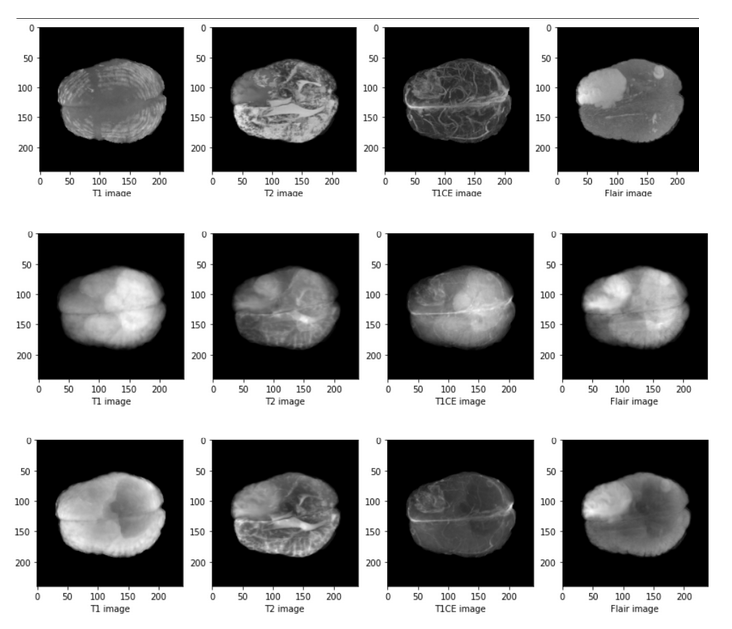
\includegraphics[height=5in]{Methodology/Chapter3Figs/3_projections.png}
    \else
      \includegraphics[bb = 92 86 545 742, height=4.5in]{3_proj}
    \fi
    \caption{\textbf{Row 1} is the Max intensity projection, \textbf{Row 2} is the Mean intensity projection and \textbf{Row 3} is the SD projection}
    \label{3_proj}
  \end{center}
\end{figure}

Classification accuracies was compared with 3 kinds of projections, as well as on 3 different axes (axial, coronal and Saggital). \textbf{EfficientNet B7} was used as a baseline model with \textbf{Focal Loss} as the loss function. Generally, EfficientNet is trained for dimensions of $(x,y,3)$ to incorporate 3-channel RGB, but in this case we used it for predicting 2D images of dimensions $(x,y,1)$.  The results are summarized in the later section \ref{volumetric_results}. 


\section{Cascaded mask-cropped model}\label{cropped_cascaded}
\vspace*{3mm}
One drawback of using the entire tumour image for classification is that it encodes redundant information. The pixels which correspond to the non-tumour tissues can be disposed. Therefore, there is a strong need for a tumour localization strategy that solves this issue. The solution is to train separate classification and segmentation models in a cascaded fashion. 
\vspace*{3mm}

The tumour localization can be done on a pre-determined 2D level or an adaptive 3D level. The 2D approach can have a large bias since the selection of the 2D slice isn't dependent upon the patient scan sample, hence ascertains no effect to the end-to-end pipeline.
\subsection{2D mask-cropped}\label{2D_cropped}
\vspace*{1mm}

\begin{figure}[H]
  \begin{center}
    \leavevmode
    \ifpdf
      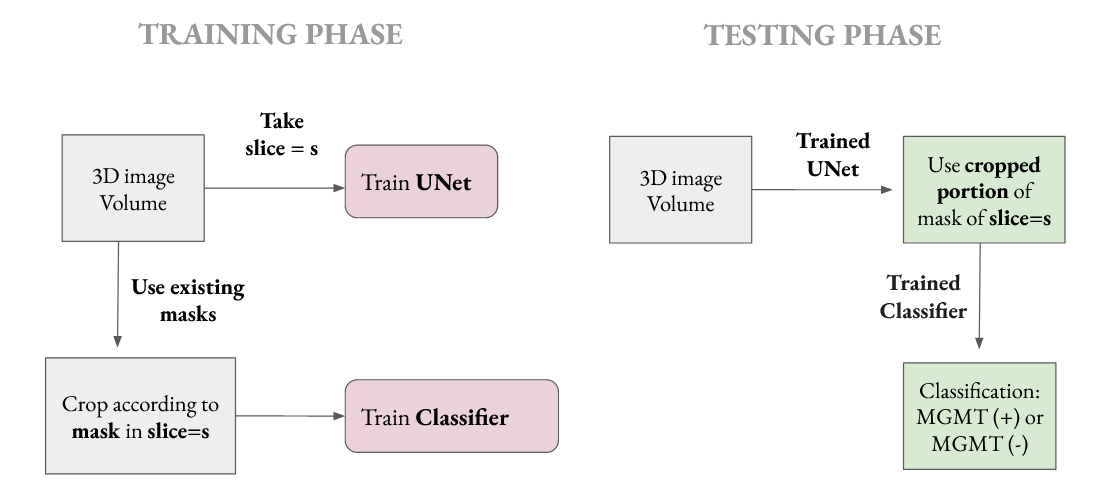
\includegraphics[height=2.5in]{Methodology/Chapter3Figs/2D_cascaded.png}
    \else
      \includegraphics[bb = 92 86 545 742, height=4.5in]{2d_cascaded}
    \fi
    \caption{Training and Testing phases of 2D model}
    \label{2d_cascaded}
  \end{center}
\end{figure}




\begin{algorithm}[H]
\caption{2D cascaded: SEGMENTATION}\label{alg:2D_cascaded_1}
\begin{algorithmic}[1]
\vspace*{4mm}
\Require Slice = s (pre-determined by user)
\For{\texttt{<Each sample in TRAIN set >}}
        \State Extract the slice = s (pre-defined)
        \State Pass that slice to UNet 
        \State Train Unet on all the slices = s 
\EndFor
\State
\For{\texttt{<Each sample in TEST set >}}
    \State Pass the slice = s to UNet
    \State Get the tumour mask
    \State Get the best-bounded-box of the tumour (crop)
    \State Save it in a separate folder
\EndFor

\end{algorithmic}
\end{algorithm}

After we have all the tumour-cropped portions of the train and test set, we move towards the Classifier training. It is to be noted that the cropped regions of the train set are directly obtained from ground-truth masks whereas the cropped regions of the test set are obtained by using the UNet predictions.
\begin{algorithm}[H]
\caption{2D cascaded: CLASSIFICATION}\label{alg:2D_cascaded_2}
\begin{algorithmic}[1]
\vspace*{4mm}
\For{\texttt{<Each sample in TRAIN set >}}
        \State Use ground-truth mask to get cropped image
        \State Pass that cropped slice to Classifier
        \State Train Classifier
\EndFor
\State
\For{\texttt{<Each sample in \textbf{cropped TEST set} >}}
    \State Pass that cropped slice to Classifer
    \State Get methylation prediction probability and output (\textbf{patient level})
\EndFor

\end{algorithmic}
\end{algorithm}
%\vspace*{2mm}

The following images show some examples with the original tumour image, the binary mask and the cropped mask region. 

\begin{figure}[H]
  \begin{center}
    \leavevmode
    \ifpdf
      \includegraphics[height=3.5in]{Methodology/Chapter3Figs/mask_cropped.png}
    \else
      \includegraphics[bb = 92 86 545 742, height=4.5in]{mask_cropped}
    \fi
    \caption{Images with their cropped masked tumours}
    \label{mask_cropped}
  \end{center}
\end{figure}

As classifier, we have used \textbf{ResNet18} and \textbf{EfficientNet B7} with Focal Loss as the classification loss function. The results are summarized in the subsequent section. However, using a pre-determined slice for the pipeline is not desired because it leads to a high bias. Hence, we move to 3D tumour localizations.

\subsection{3D mask cropped}\label{3D_cropped}
\vspace*{4mm}
The 3D tumour localization version takes into account a 3D stacked tumour voxel instead of just a single slice. The central location of the voxel (from the 155 slices) is judged according to the tumour visibility of the slices. The slice with the best tumour visibility is chosen as the middle slice and other slices are taken around it. The tumour visibility is judged by the percentage of '1' labelled pixels in the predicted mask. 

\begin{figure}[H]
  \begin{center}
    \leavevmode
    \ifpdf
      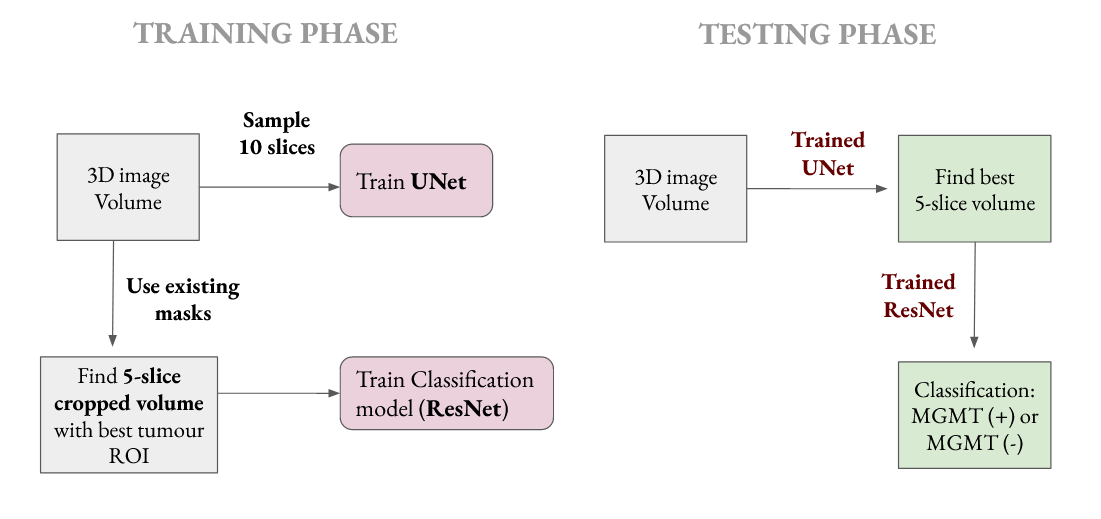
\includegraphics[height=2.7in]{Methodology/Chapter3Figs/cascaded_training_testing.png}
    \else
      \includegraphics[bb = 92 86 545 742, height=4.5in]{3d_cascaded}
    \fi
    \caption{Training and Testing phases of 3D volume model}
    \label{3d_cascaded}
  \end{center}
\end{figure}

After repeated experimentation across all 3 axes (axial, coronal and sagittal) we decided to use a \textbf{5-slice volume} for the 3D localization of the tumour. The middle slice from the 5-sliced stack has the best tumour visible and 2 slices each are chosen from the top and bottom of the chosen best slice.

\begin{algorithm}[H]
\caption{3D cascaded: SEGMENTATION}\label{alg:3D_cascaded_1}
\begin{algorithmic}[1]
\vspace*{2mm}
\For{\texttt{<Each sample in TRAIN set >}}
        \State Sample \textbf{10 slices} (except from top 20\% and bottom 20\% slices)
        \State Train Unet on all the sampled slices 
\EndFor
\For{\texttt{<Each sample in TEST set >}}
    \State Pass \textbf{each slice} to UNet
    \State Get the tumour mask for each slice individually
    \State Find the best slice with most tumour visible, Say $slice = x$
    \State Crop the tumour portions from slices $[x-2, x-1,x,x+1,x+2]$ to get 5-stacked volume
    \State Save 5-stacked volume in a separate folder
\EndFor

\end{algorithmic}
\end{algorithm}
\vspace*{2mm}
\begin{algorithm}[H]
\caption{3D cascaded: CLASSIFICATION}\label{alg:3D_cascaded_2}
\begin{algorithmic}[1]
\vspace*{4mm}
\For{\texttt{<Each sample in TRAIN set >}}
        \State Use ground-truth mask (slice-by-slice) to get $slice=a$ with best tumour visibility
        \State Crop the tumour portions from slices $[a-2, a-1,a,a+1,a+2]$ to get 5-stacked volume
        \State Pass that 3D volume to Classifier
        \State Train Classifier
\EndFor
\State 
\For{\texttt{<Each sample in \textbf{3D cropped TEST set} >}}
    \State Pass that 3D 5-stacked volume to Classifer
    \State Get methylation prediction probability and output (\textbf{patient level})
\EndFor

\end{algorithmic}
\end{algorithm}
\vspace*{4mm}
The benefit of extending the 2D slice version to a 3D volume version is that the pipeline now decides which tumour slice to extract the most information from. A quick iteration across all the given datapoints told us that the tumour location is fairly variable and hence using a pre-set slice is not the best option. Also, training the Unet on 10 samples from each patient scan makes the segmentation more robust for unseen data.
\vspace*{4mm}

The 3D version was tried with various models (across all the 3 axes): \textbf{ResNet18, ResNet34}, the EfficientNet model group (\textbf{EfficientNet B0,EfficientNet B3, EfficientNet B7}. Ensembles of ResNet18 + ResNet34 and ResNet + EfficientNet was also experimented with. The AUCs and accuracies are presented in section \ref{cropped_results}.
\\
\\
\\
\subsection{Ensemble along 3 axes}\label{3-axis-ensemble}
\vspace*{4mm}

The final part of our methodology involved using a 3-axis-ensemble, in which the same patient scan is utilized along the 3 axes (by using 3 separately trained UNet and 3 separately trained Classifiers) and the final predictions are ensembled together to get the final prediction probability. The same 3D MRI scan is sampled along the 3 axis to train the Unet and then used sliced by slice (in testing phase) to get the 5-stack volume which has the best tumour visibility along that particular axis.
\vspace*{4mm}
\begin{figure}[H]
  \begin{center}
    \leavevmode
    \ifpdf
      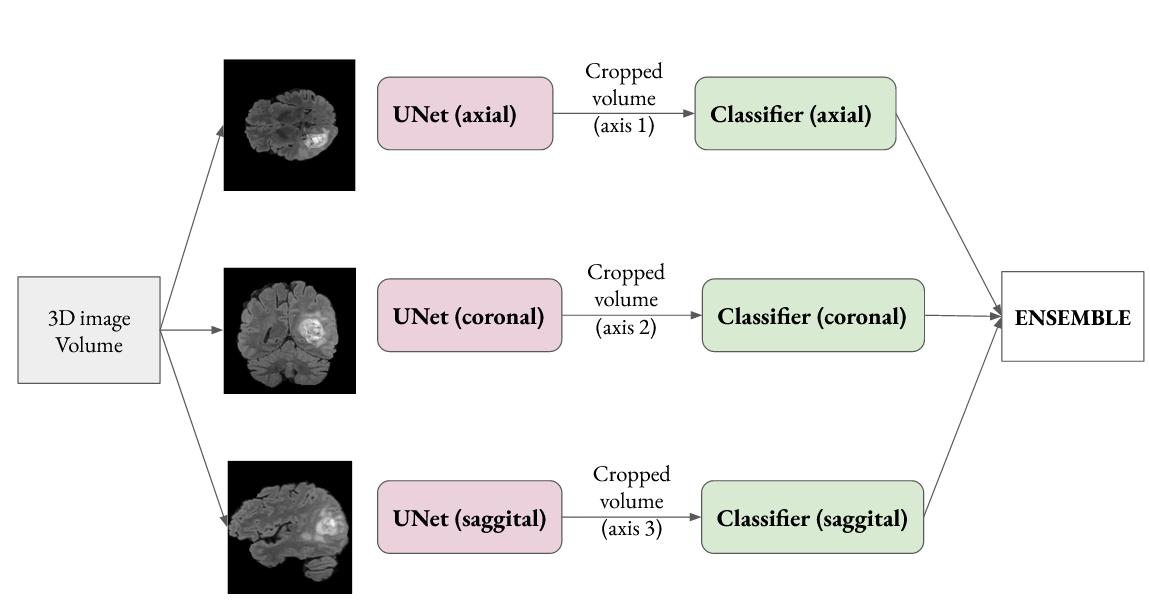
\includegraphics[height=3.2in]{Methodology/Chapter3Figs/3_axis_ensemble.png}
    \else
      \includegraphics[bb = 92 86 545 742, height=4.5in]{3axis}
    \fi
    \caption{3-axis 3D volume classifier ensemble}
    \label{3axis}
  \end{center}
\end{figure}

The classifiers used in each case for each branch was \textbf{ResNet18} and \textbf{ResNet34} since they were lighweight. The number of model parameters becomes three times due to the increased branches of axis 2 and axis 3. The results of the ensemble are shown in section \ref{3_axis_results}.














% ------------------------------------------------------------------------


%%% Local Variables: 
%%% mode: latex
%%% TeX-master: "../thesis"
%%% End: 
